\chapter{绘制端盖立体图}

{\bfseries 知识目标}
\begin{itemize}
\item 掌握
\end{itemize}

{\bfseries 技能目标}
\begin{itemize}
\item 能够运行
\item 能够运行
\end{itemize}

{\bfseries 本单提要}

本章通过完成端盖块零件的立体图绘制,使读者能够掌握圆角命令的使用,能够针对复杂的回转体块零件进行绘图分析,选择适当的建模方法来加速零件的建模。图\ref{fig:tiaoyafaduangai}所示即为本章要完成的任务。
\noindent
\begin{figure}[htbp]
\centering
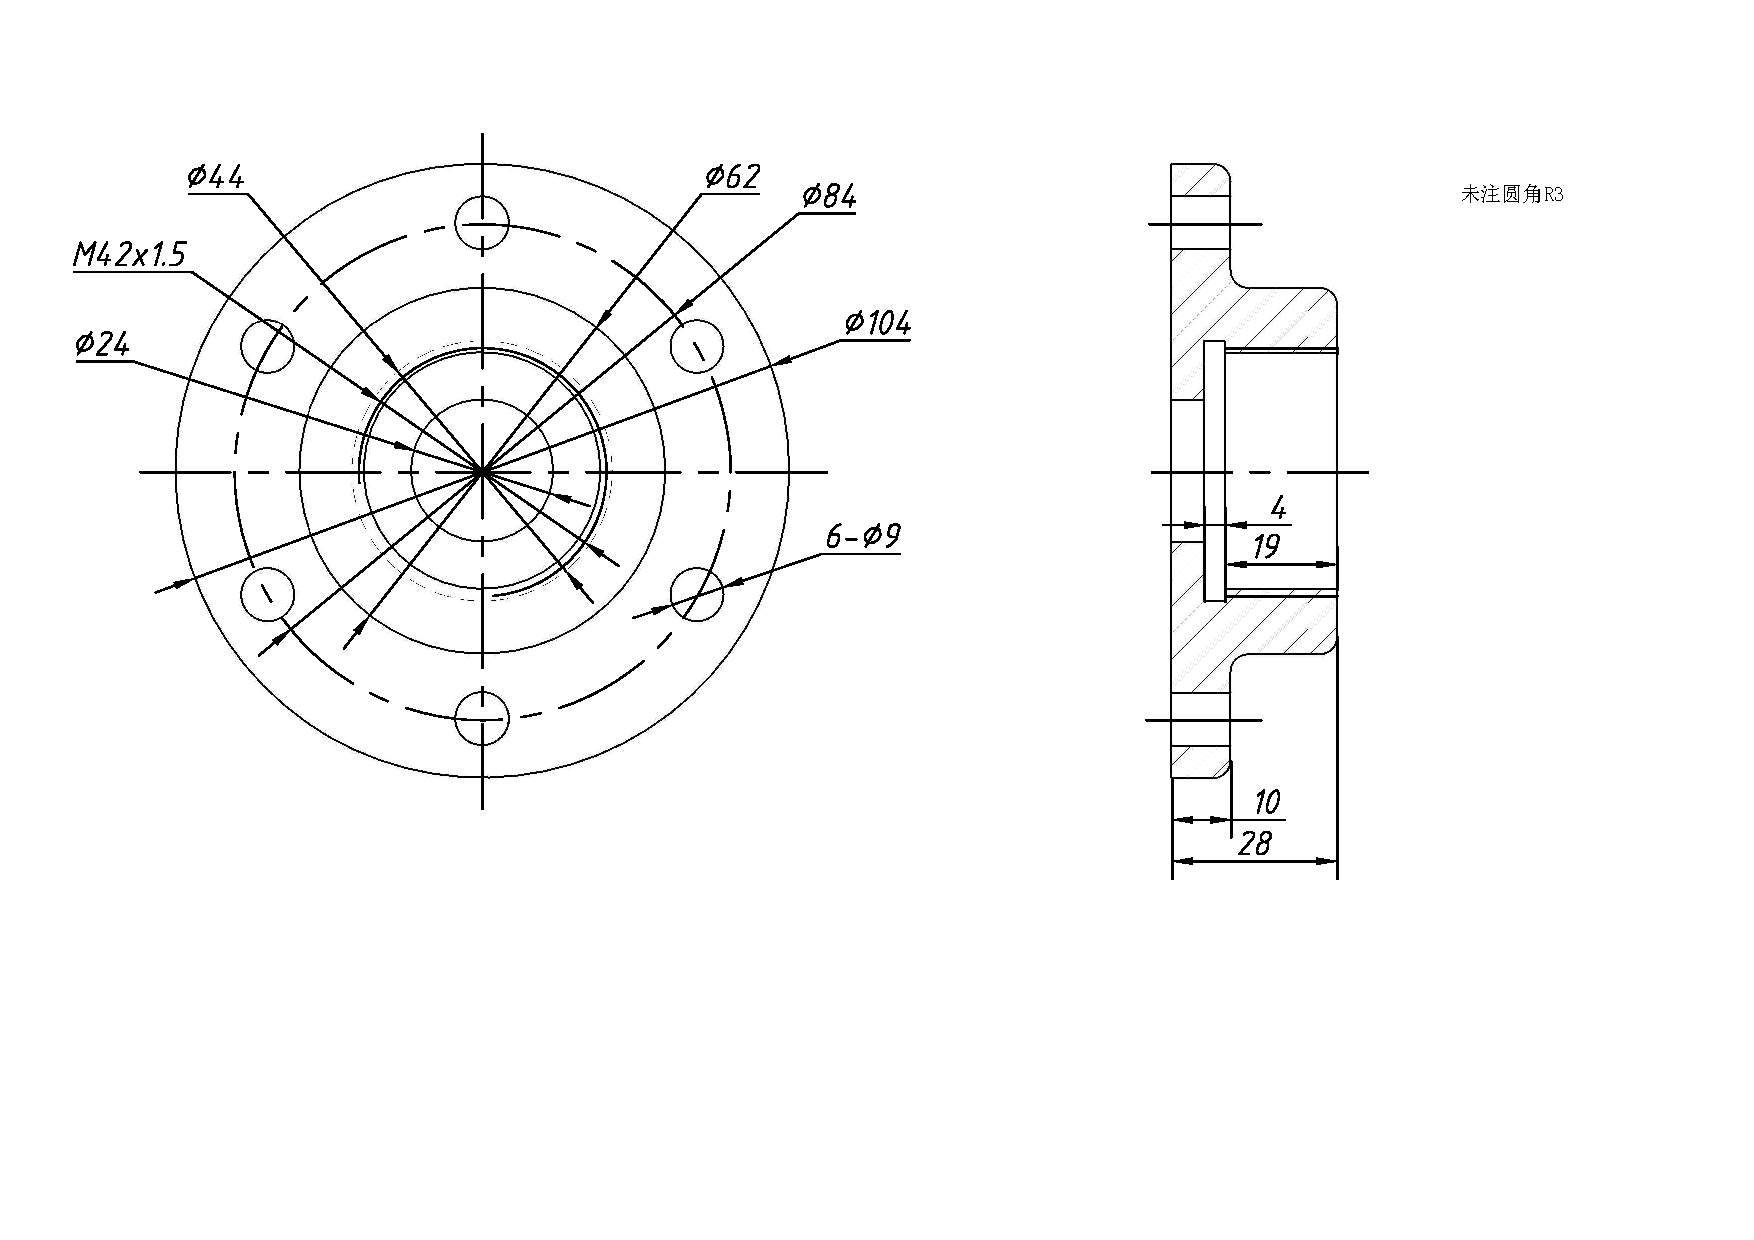
\includegraphics[scale=0.5]{tiaoyafaduangai.pdf}
\caption{端盖零件图}\label{fig:tiaoyafaduangai}
\end{figure}
\endinput